  \section[International Classification of Diseases (ICD) ]{ICD}
  \label{sec:icd}

  \initial{I}\textit{nternational Classification of Diseases (ICD)}\
  is a classification of diseases by WHO to permit the systematic recording, analysis,\
  interpretation and comparison of mortality and morbidity data collected in\
  different countries or areas and at different times. The ICD is used to\
  translate diagnoses of diseases and other health problems from words into an\
  alphanumeric code, which permits easy storage, retrieval and analysis of the data.\
  In practice, the ICD has become the international standard diagnostic classification\
  for all general epidemiological and many health management purposes.\\
  
  \noindent The ICD can be used to classify diseases and other health problems recorded on\
  many types of health and vital records. Its original use was to classify causes of\
  mortality as recorded at the registration of death. Later, its scope was extended\
  to include diagnoses in morbidity. It is important to note that, although the\
  ICD is primarily designed for the classification of diseases and injuries with\
  a formal diagnosis, not every problem or reason for coming into contact with\
  health services can be categorized in this way. Consequently, the ICD provides\
  for a wide variety of signs, symptoms, abnormal findings, complaints and social\
  circumstances that may stand in place of a diagnosis on health-related records.\
  It can therefore be used to classify data\
  recorded under headings such as `diagnosis', `reason for admission', `conditions\
  treated' and `reason for consultation', which appear on a wide variety of health\
  records from which statistics and other health-situation information are derived.\\
  
  \subsection{Family of Diseases}
  \begin{figure}[!ht]
    \centering
    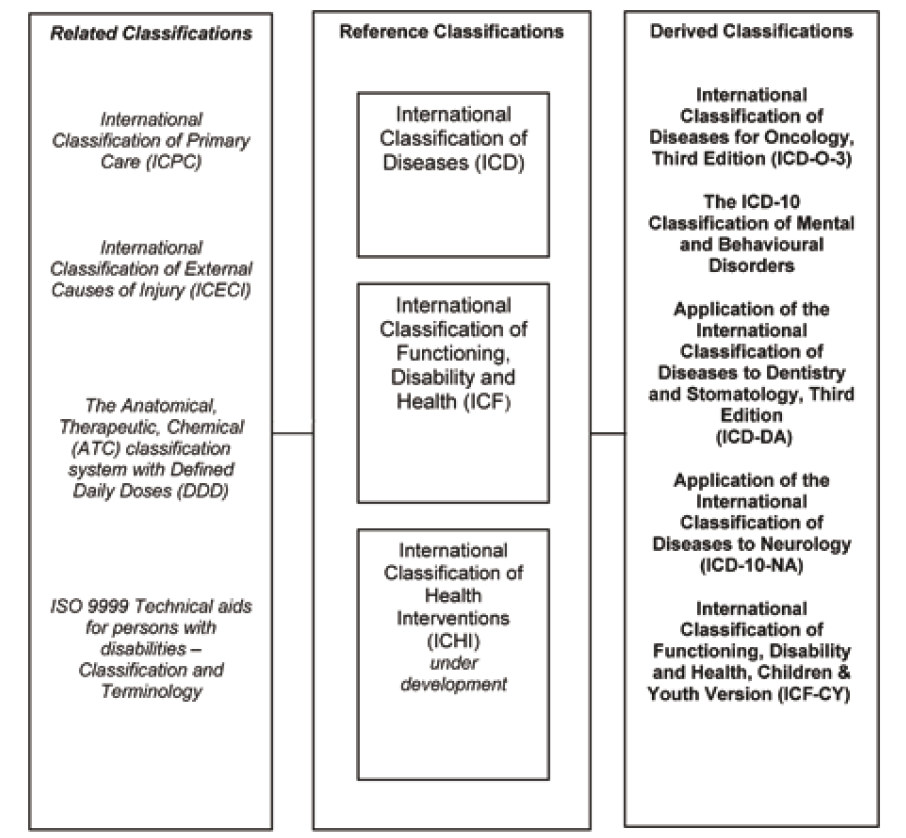
\includegraphics[width=\textwidth]{icd_fic.png}
    \caption{Schematic representation of the WHO-FIC\
    \citep{icd10_instruction_manual_-_volume_2_international_2010}}
    \label{fig:icd_fic}
  \end{figure}
  Although the ICD is suitable for many different applications, it does not serve\
  all the needs of its various users. It does not provide sufficient detail for some\
  specialties and sometimes information on different attributes of health conditions\
  may be needed. The ICD also is not useful to describe functioning and disability\
  as aspects of health, and does not include a full array of health interventions or\
  reasons for encounter. In order to overcome these shortcomings, the concept of\
  \emph{family of diseases} was developed.\
  Currently `family' designates a suite\
  of integrated classification products that share similar features and can be used\
  singularly or jointly to provide information on different aspects of health\
  and health-care system. For example, the ICD as a reference classification is\
  mainly used to capture information on mortality and morbidity. Additional aspects\
  of health domains, functioning and disability have now been jointly classified\
  in the International Classification of Functioning, Disability and Health (ICF).\
  The WHO Family of International Classifications (WHO-FIC) attempts to serve\
  as the framework of international standards to provide the building blocks of\
  health information systems. Figure~\ref{fig:icd_fic} represents the types of\
  classifications in the WHO-FIC.\\
  
  \noindent Compared with ICD-9, ICD-10 has~\citep{disantostefano_international_2009}:
  \begin{itemize}
    \itemsep0ex
    \item Expanded detail for many conditions (e.g., viral hepatitis has been expanded\
    from ICD-9 070, a single 3-digit category, to ICD-10 B15-B19), five 3-digit\
    categories.\
    \item Transferred conditions around the classification (e.g., hemorrhage has\
    been moved from the circulatory chapter to the symptoms and signs chapter).\
    \item Used alphanumeric codes instead of numeric codes (e.g., code for\
    diabetes mellitus was 250.XX in ICD-9 and is E10-E14 in ICD-10).
    \item Modified coding rules (e.g., the ``Old pneumonia, influenza and maternal\
    conditions'' and ``Error and accidents in medical care'' coding rules have\
    been eliminated).\
    \item Modified the tabulation lists (e.g., the U.S. ICD-10 113-clause list replaces\
    the U.S. ICD-9 72-cause list).
  \end{itemize}
  
  \noindent  A comprehensive list of resources can be accessed on the WHO-ICD\
  website\footnote{\url{http://www.who.int/classifications/icd/en/}}. One of the\
  interesting tools in an online application designed for classroom training as\
  well as self-training on ICD-10.
  
  